\section{Arquitectura}
\label{sec:Prop_Arquitectura}


EN ALGÚN LADO DEBO DESCRIBIR EL PROCESO DE FILTRADO



% A partir de dos arquitecturas relevantes para este trabajo \cite{otebolaku2015context} \cite{miso2012highly}, se propone la arquitectura general del sistema que se puede observar en la Figura  \ref{fig:Diagrama_General}, a continuación se presentan los componentes y una breve descripción de cada uno.


\begin{figure}[ht]
\centering%
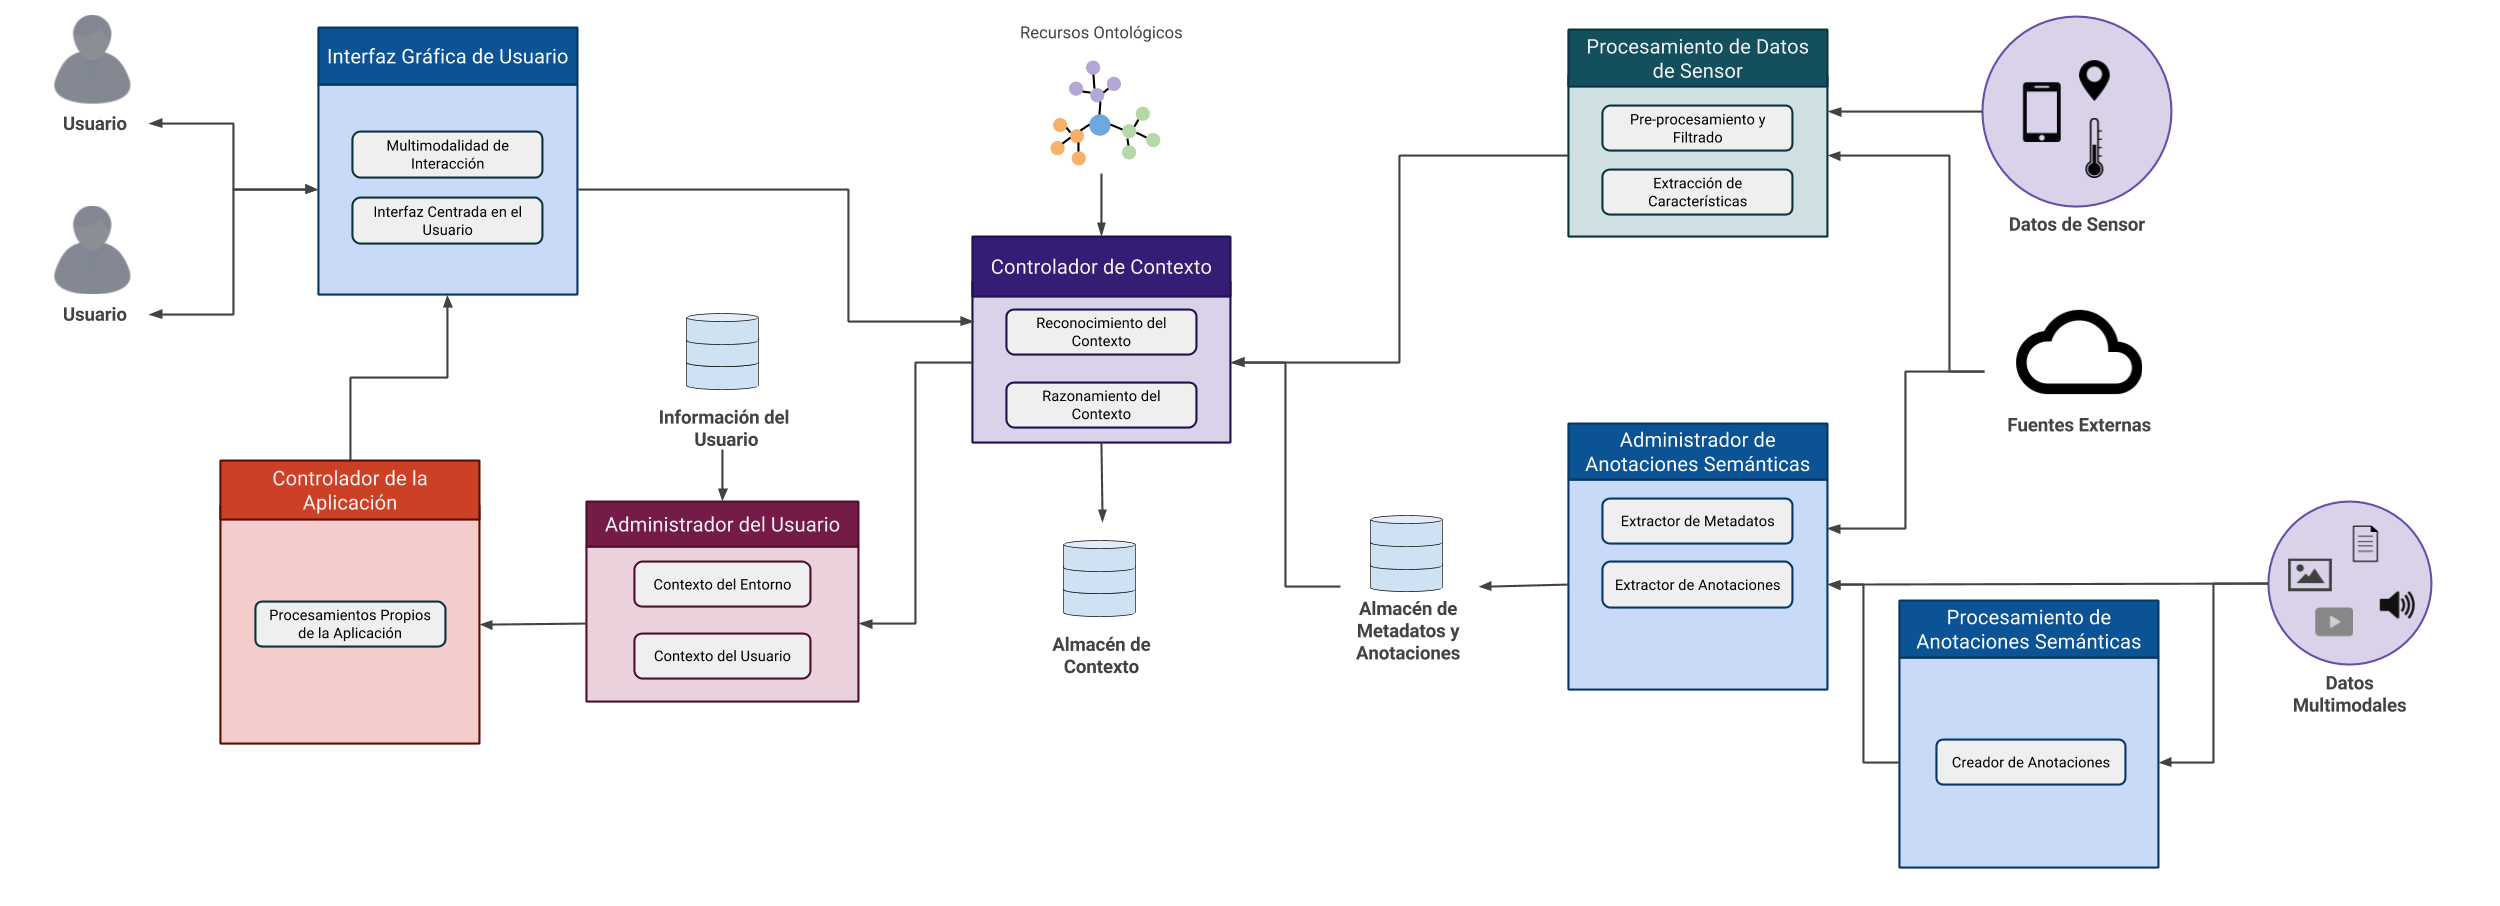
\includegraphics[width=\textwidth]{Cap3/Images/Diagrama_General}%
\caption{Diagrama general del sistema sensible al contexto multimodal.} \label{fig:Diagrama_General}
\end{figure}

% Antes de empezar con la descripción de la arquitectura se deben definir algunos términos: (i) Ítem: Cualquier elemento que pueda ser sugerido al usuario, puede ser un objeto por comprar, un lugar por visitar o una actividad por desarrollar, (ii) etiqueta: es el texto asociado a un contenido multimedia, (iii) anotación: texto que se asocia solo a una parte del contenido \cite{bracamonte2017extracting}. También es necesario definir un lenguaje de marcado que permita la interoperabilidad entre plataformas como XML o RDF \cite{nanarvaez2016modelo, barnaghi2013linked}.

% \begin{enumerate}

% \item Datos Multimodales: Son datos capturados en diferentes formatos por los usuarios, pueden tener algún tipo de relación por localización o por fecha de captura, y se obtienen por medio de un dispositivo de interacción.
% \item Datos de Sensor: Se obtienen a partir de redes de sensores que tienen acceso a internet y que describen las características del entorno de una entidad.
% \item Fuentes externas: Son datos que no son creados por el usuario ni son capturados con dispositivo de interacción, pueden describir el estado de una entidad o proveer información adicional que ayude a obtener el contexto.
% \item Administrador de Datos Multimodales (ADM): Su propósito es obtener la información para la creación de los objetos archivo y multimedia propuestos por Narvaez et al. [15], tiene en cuenta etapas de extracción de metadatos, anotaciones y etiquetas. Para realizar las etiquetas y anotaciones se pueden usar estrategias manuales, semiautomáticas o automáticas. 
% \item Administrador de Datos del Sensor (ADS): Procesa la información obtenida de los sensores eliminando datos atípicos. Adicionalmente, utiliza estrategias de clasificación para identificar automáticamente la acción que desarrolla un usuario. Tanto el ADM como el ADS envía anotaciones textuales que serán analizadas por el Administrador de Contexto.
% \item Almacén de Metadatos y Anotaciones: Dado que obtener las características de los contenidos cada vez que el usuario lo requiera es costoso, cuando se registra un nuevo contenido el ADM lo procesa y los resultados son almacenados en este componente. Mientras que los datos de sensor son analizados en tiempo real, los datos multimodales serán analizados una vez y podrán ser actualizados.
% \item Recursos Ontológicos: Las ontologías son el modelo de representación recomendado en este trabajo. Según Perera et al. [6] las ontologías permiten el intercambio de información entre sistemas y facilitan el proceso de razonamiento sobre las variables de contexto, se recomienda combinar estrategias de razonamiento para hacer el algoritmo mucho más confiable.
% \item Administrador de Contexto: Realiza los llamados al ADM y ADS para obtener las variables de contexto, y realiza procesos de razonamiento logrando que el sistema actúe automáticamente en la recomendación. Las ontologías, son la fuente principal de información para el modelado y razonamiento de contexto en esta propuesta.
% \item Administrador del Usuario: Procesa la información del usuario y el entorno para seleccionar el contexto más adecuado según sus preferencias e historial de actividades desarrolladas.
% \item Información del Usuario: Almacena la información personal del usuario y sus preferencias en ítems y contexto.
% \item Sistema de Recomendación: Obtiene los datos de los ítems que se pueden usar en el proceso de recomendación, como se indicó en la sección 2.3 el tipo de recomendación puede variar dependiendo de la calidad, cantidad y tipo de datos de los que se disponga; y de la aplicación que se va a dar al sistema. Luego los datos se filtran de acuerdo a la información contextual identificada y finalmente se realiza la recomendación.
% \item Contenidos del Dominio: Es la información de los ítems que serán analizados y recomendados por el sistema.
% \item Usuario: Quien desea obtener una recomendación por parte del sistema.


% \end{enumerate}

\subsection{Multimedia Context}
\label{sec:Prop_MultimediaContext}